% Tento soubor nahraďte vlastním souborem s přílohami (nadpisy níže jsou pouze pro příklad)
% This file should be replaced with your file with an appendices (headings below are examples only)

% Umístění obsahu paměťového média do příloh je vhodné konzultovat s vedoucím
% Placing of table of contents of the memory media here should be consulted with a supervisor

\chapter{Obsah přiloženého paměťového média}

\begin{itemize}
    \item \texttt{src} -- Zdrojové kódy vytvořené aplikace \texttt{WarehouseManager}.
    \item \texttt{utils} -- Skripty používané v~průběhu práce, zejména ke trénování na výpočetním clusteru a~k~vyhodnocení.
    \item \texttt{doc} -- Plakát použitý k prezentaci této práce a video prezentující dosažené výsledky.
    \item \texttt{README} -- Více obsáhlá příručka v~anglickém jazyce (ve formátu \texttt{md} -- \emph{markdown}).
    \item \texttt{report} -- Adresář obsahující zdrojové kódy tohoto dokumentu ve formátu \LaTeX, a~také jejich přeloženou verzi ve formátu \texttt{PDF}.
\end{itemize}


\chapter{Manuál}

Sestavení a použití aplikace \texttt{WarehouseManager} na linuxovém OS:

\begin{enumerate}
    \item Instalace grafického frameworku \texttt{Qt5} a knihovny \texttt{SIMLIB/C++} dle jejich dokumentace.
    \item Spuštění kompilace pomocí příkazu \texttt{make} v kořenovém adresáři projektu.
    \item Nastavení konfigurace v grafickém rozhraní nebo v souborech v adresáři \texttt{cfg/}.
    \item Po úspěšné kompilaci lze provést spuštění nástrojů následovně:
    \begin{verbatim}
        ./whm_gui
        ./whm_gen -o orders.xml -a articles.csv
        ./whm_sim -o orders_test.xml  -i locations.csv \
                  -l layout.xml
        ./whm_paf -o orders_test.xml  -i locations.csv \
                  -l layout.xml [-s]
        ./whm_opt -o orders_train.xml -i locations.csv \
                  -l layout.xml -a articles.csv -O 1-6
    \end{verbatim}
    \item Data pro testování lze najít v adresáři \texttt{data/} a jeho podadresářích.
    \item Výsledky lze při použití příkazové řádky vidět na standardním výstupu a v případě použití grafické aplikace přímo v ní.
    \item Pro více informací lze nahlédnout do \texttt{README} nebo vyvolat pomoc přepínačem \texttt{-h}.
\end{enumerate}

\chapter{Plakát}
\begin{center}
    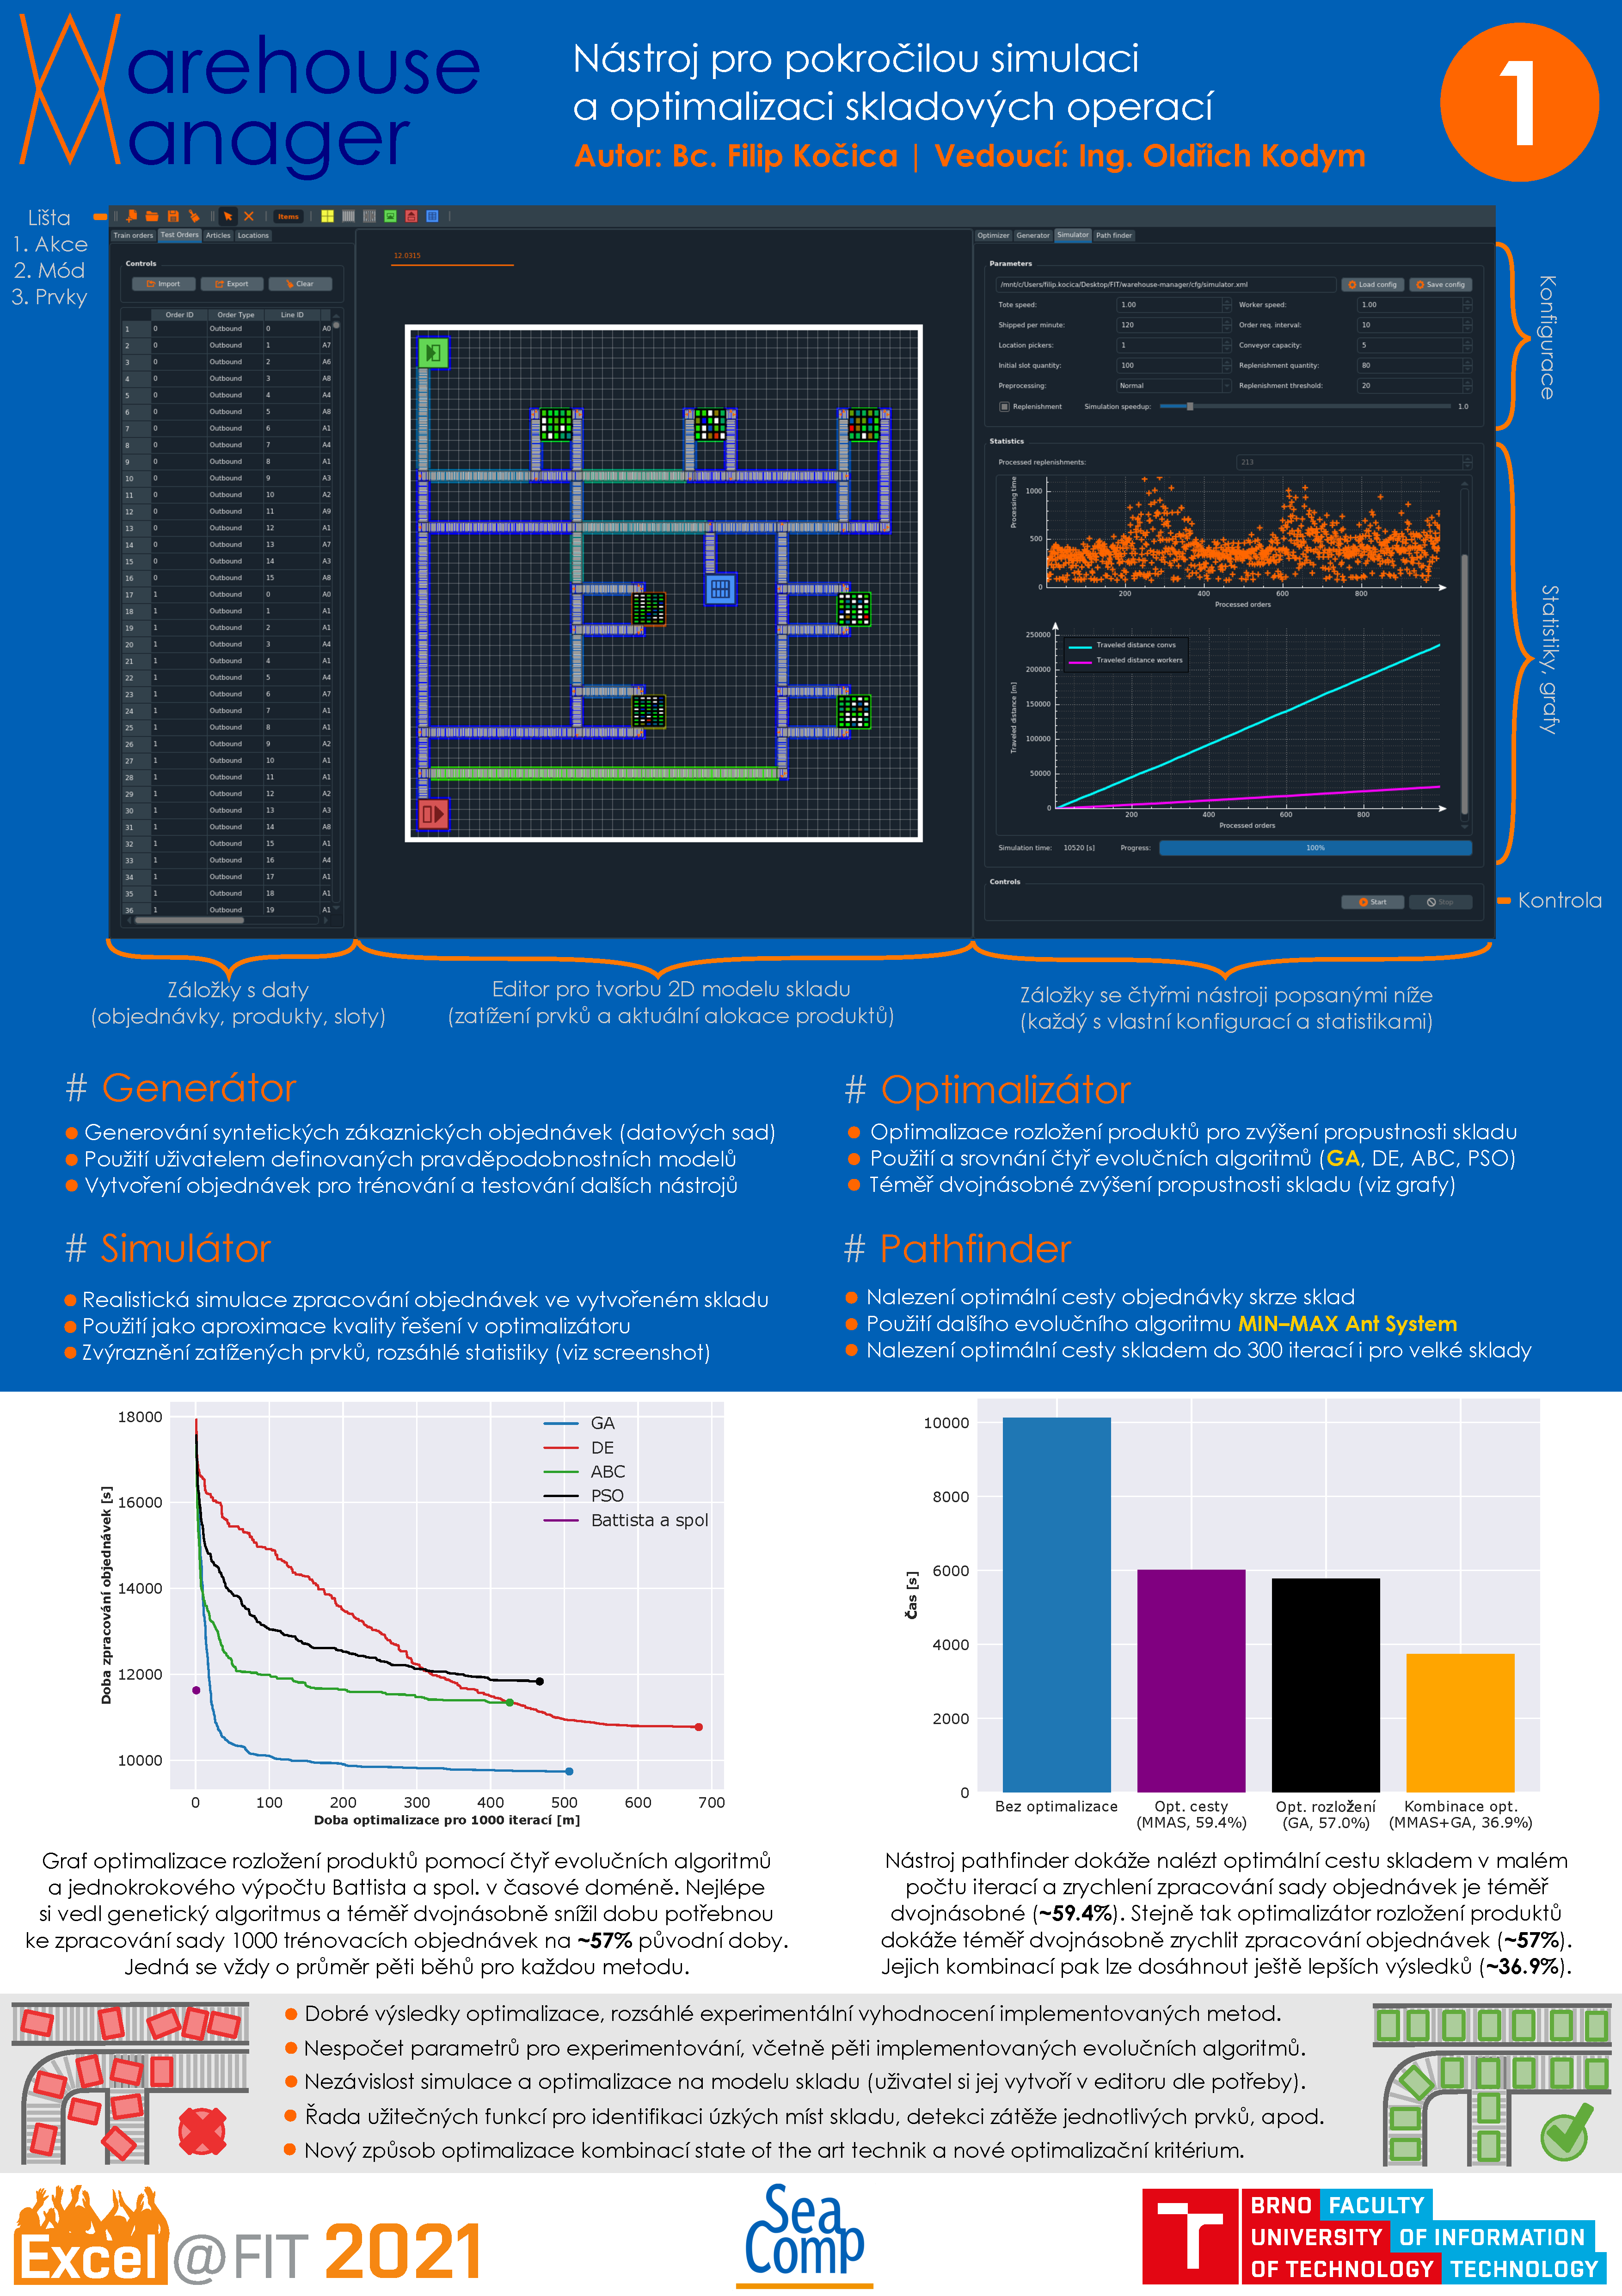
\includegraphics[width=0.75\linewidth]{figures/prilohy/poster.pdf}
\end{center}